\documentclass[11pt]{article}
\usepackage{graphicx}

\title{NRR-Guarantee: Bounded Commit/Defer Guarantee Surfaces and Explicit Downstream Boundaries}
\author{Kei Saito}
\date{April 2, 2026}

\begin{document}
\maketitle

\begin{abstract}
This manuscript sets the current downstream \texttt{Guarantee} surface for the
Non-Resolution Reasoning (NRR) program. Its purpose is to close the next paper
as a bounded claim layer rather than as a broad universality paper. Under
explicit provider, family, horizon, and observability conditions, the current
manuscript integrates one supported claim surface, one downstream-acceptance
boundary surface, one side-topic supporting surface, and one later-horizon
boundary surface: frozen early ambiguity-turn resolution, downstream
acceptance under the inherited mainline comparison contract, repaired
first-step side-topic/quarantine workstart, and later-horizon
relation-preservation failure reporting. On the current tested-provider
surface, the early ambiguity-turn read moves from \texttt{0 / 24} to
\texttt{24 / 24} on both providers for
\texttt{resolution\_attempt\_present} and \texttt{appropriate}, and from
\texttt{8 / 24} to \texttt{24 / 24} for
\texttt{unilateral\_commit\_absent}; the repaired downstream-acceptance boundary supports bounded
\texttt{preacceptance\_rework\_burden\_absent} improvement under matched
\texttt{baseline vs Energy policy} conditions (both provider slices move from
\texttt{0 / 24} to \texttt{24 / 24}, while Gemini
\texttt{accepted\_direction\_followthrough\_present} drops from
\texttt{13 / 24} to \texttt{10 / 24}), the auxiliary repaired
\texttt{NRR vs Ablation} read remains mixed
(\texttt{Anthropic = inconclusive}, \texttt{Gemini = support}; Anthropic
\texttt{Baseline} remains stronger than Anthropic \texttt{NRR} on
\texttt{appropriate}), and the
repaired first-step side-topic surface reaches \texttt{12 / 12} on both
providers. That side-topic surface is carried only as bounded supporting
evidence because it depends on a local repaired
\texttt{baseline vs revised Energy policy} comparison rather than on the
paper-level mainline \texttt{baseline vs Energy policy} contract. The result is
a narrow downstream paper surface: one supported guarantee claim plus explicit
downstream, side-topic, and later-horizon limits. Across those surfaces, the
honest read is therefore non-uniform: the
downstream-acceptance boundary remains provider-sensitive beyond its shared
burden-removal gain, and the later-horizon material remains boundary-only
rather than an additional supported guarantee.
\end{abstract}

\section{Introduction}

NRR is not an anti-LLM framework. NRR does not replace standard LLM use. NRR
optimizes when to commit and when to defer, under explicit conditions.

Related work in mixed-initiative and task-oriented dialogue has long examined
adaptive initiative control and goal-oriented interaction management
~\cite{chucarroll2000mimic,wen2017taskdialogue}, while clarification-focused lines
study how a system should ask follow-up questions when a user's request remains
ambiguous or underspecified~\cite{deboni2003clarification,rao2018evpi,hu2020interactive}. Grounding-oriented work further emphasizes that dialogue systems
must recover collaboratively when interpretation is not yet fixed
~\cite{benotti2021groundedclarifications,benotti2021grounding}. More recent
LLM-centered work has also revisited clarification under query ambiguity and
abstention or withholding under uncertainty
~\cite{sahay-etal-2025-ask,wen-etal-2025-know,madhusudhan-etal-2025-llms}.
Work on verified AI and runtime assurance frames a complementary question:
what scoped assurances can be justified under explicit assumptions, monitors,
and failure boundaries rather than by unconstrained behavioral optimism
~\cite{seshia2022verifiedai,desai2019soter}. The present manuscript uses
\texttt{Guarantee} in that bounded verification/assurance sense: not as a
theorem-level or provider-universal correctness claim, but as a conditioned
claim surface whose provider scope, horizon scope, observability scope, and
failure boundaries are made explicit and auditable.

Within the NRR series, \texttt{Core} and \texttt{Phi} fixed the upstream
position-dependent identity and state-mapping surfaces~\cite{saito2025nrr,saito2026phi}.
\texttt{IME}, \texttt{Transfer}, and \texttt{Coupled} then constrained the
interface, transfer, and dependency surfaces~\cite{saito2026ime,saito2026transfer,saito2026coupled}.
Integrated \texttt{paper7} fixed the manuscript-facing delayed-commitment
comparison and boundary-honesty surface, and \texttt{Energy} fixed the current
calibration/control handoff that the present manuscript now inherits as its
direct upstream spine~\cite{saito2026principles,saito2026energy}.

The present manuscript instead treats \texttt{Policy}, \texttt{Dynamics}, and
\texttt{Policy-Verification} as manuscript-facing supporting layers for a
bounded \texttt{Guarantee} read rather than as independent completion targets
or a serial upstream chain. Accordingly, its purpose is to state only those
downstream surfaces that remain supportable when the manuscript-facing
dependency spine is kept at \texttt{paper7 -> Energy -> Guarantee} and when
provider, family, horizon, observability, and failure-boundary limits are made
explicit.

The Core-to-Guarantee program goal itself is not being rewritten here. What the
series must establish from \texttt{Core} through \texttt{Guarantee} remains the
same: a framework grounded in position-dependent identity as a first principle,
closed as an engineering program of conditional utility through
implementation, quality measurement, operational control, and verification. The
current \textit{non-evaluative principle} read reorganizes that same program; it
does not replace the top-level goal. In this manuscript, the practical use of
that read is to tighten closure discipline around a narrow notion of
`evaluation', namely full branchwise comparative evaluation during retention.

The present version is intentionally narrow. It states the currently supported
bounded claim surface without promoting any unverified provider-universal,
family-universal, or long-horizon statement.

\paragraph{Series Consistency Statement:}
Unsupported interpretations are never injected at a fixed evidence state,
hypothesis-set expansion is evidence-gated, and unobserved possibilities remain
explicitly unresolved. In this paper, the evidence-source clause is restricted to
the frozen downstream support layers and the directly imported observability
surfaces named for the current \texttt{Guarantee} manuscript line.

\paragraph{Series Extensibility Statement:}
NRR is a derivation-and-evaluation framework, not a closed recipe. The currently
evaluated policy/operator set is treated as an evaluated set under tested
conditions, not as an exhaustive set. The aim of the present manuscript is not
to imply that the current runs exhaust the guarantee question, but to fix a
reusable test surface: one bounded supported claim, explicit supporting and
boundary surfaces, explicit comparison rules, provider-sliced reporting, and
visible failure boundaries that later readers can rerun, challenge, and extend
under new providers, new families, and longer horizons.

\section{Contributions}

Under the currently fixed provider, family, horizon, and observability bounds,
this manuscript makes four bounded contributions:

\begin{enumerate}
\item it establishes bounded early ambiguity-turn support for non-unilateral
priority resolution under matched \texttt{baseline vs Energy policy}
conditions;
\item it carries downstream acceptance as an explicit boundary surface: the
mainline \texttt{baseline vs Energy policy} comparison supports shared
\texttt{preacceptance\_rework\_burden\_absent}, while visible provider-sliced
residuals prevent pair-wide downstream-quality closure;
\item it carries repaired first-step side-topic / quarantine evidence as a
bounded supporting surface under matched
\texttt{baseline vs revised Energy policy} conditions, with the main
incremental lift concentrated in \texttt{C\_incident\_response} and without
upgrading that local repaired comparison into a second manuscript supported
claim;
\item it keeps later-horizon degradation and unsupported extensions explicit as
failure-boundary reporting and reusable rerun surfaces rather than inflating
them into broader guarantee language.
\end{enumerate}

\section{Program Position And Scope}

This paper sits at the end of the current manuscript-facing downstream spine:

\begin{center}
\texttt{paper7 -> Energy -> Guarantee}
\end{center}

\noindent The manuscript-facing dependency split is fixed for interpretation.
Integrated \texttt{paper7} supplies the comparison-and-boundary-honesty
upstream surface. \texttt{Energy} supplies the calibration/control handoff and
the current imported evidence surface.
\texttt{Policy} supplies the minimal state/action specification.
\texttt{Dynamics} supplies the hold/degrade/break vocabulary over later
checkpoints. \texttt{Policy-Verification} supplies the prospective matched-
condition validation surface. \texttt{Guarantee} then carries the bounded
supported, supporting, and boundary surfaces that remain after those inputs are
imported under explicit conditions.

This means the manuscript has a double obligation. It must absorb the already
fixed supporting layers without reopening their ownership boundaries, and it must
state only those guarantee-shaped claims that remain supportable after explicit
restriction of provider, family, horizon, observability, and failure boundary.

The current organizing read is likewise narrow. The
\textit{non-evaluative principle} is used here only as a local way to organize
what counts as satisfactory closure for this manuscript, not as a theorem-level
claim that supersedes the Core-to-Guarantee objective itself. In that narrower
sense, \texttt{Guarantee} is the downstream line where the bounded supported,
supporting, and boundary surfaces must be stated without inflating them into
unrestricted runtime branchwise comparison.

\begin{figure}[ht]
\centering
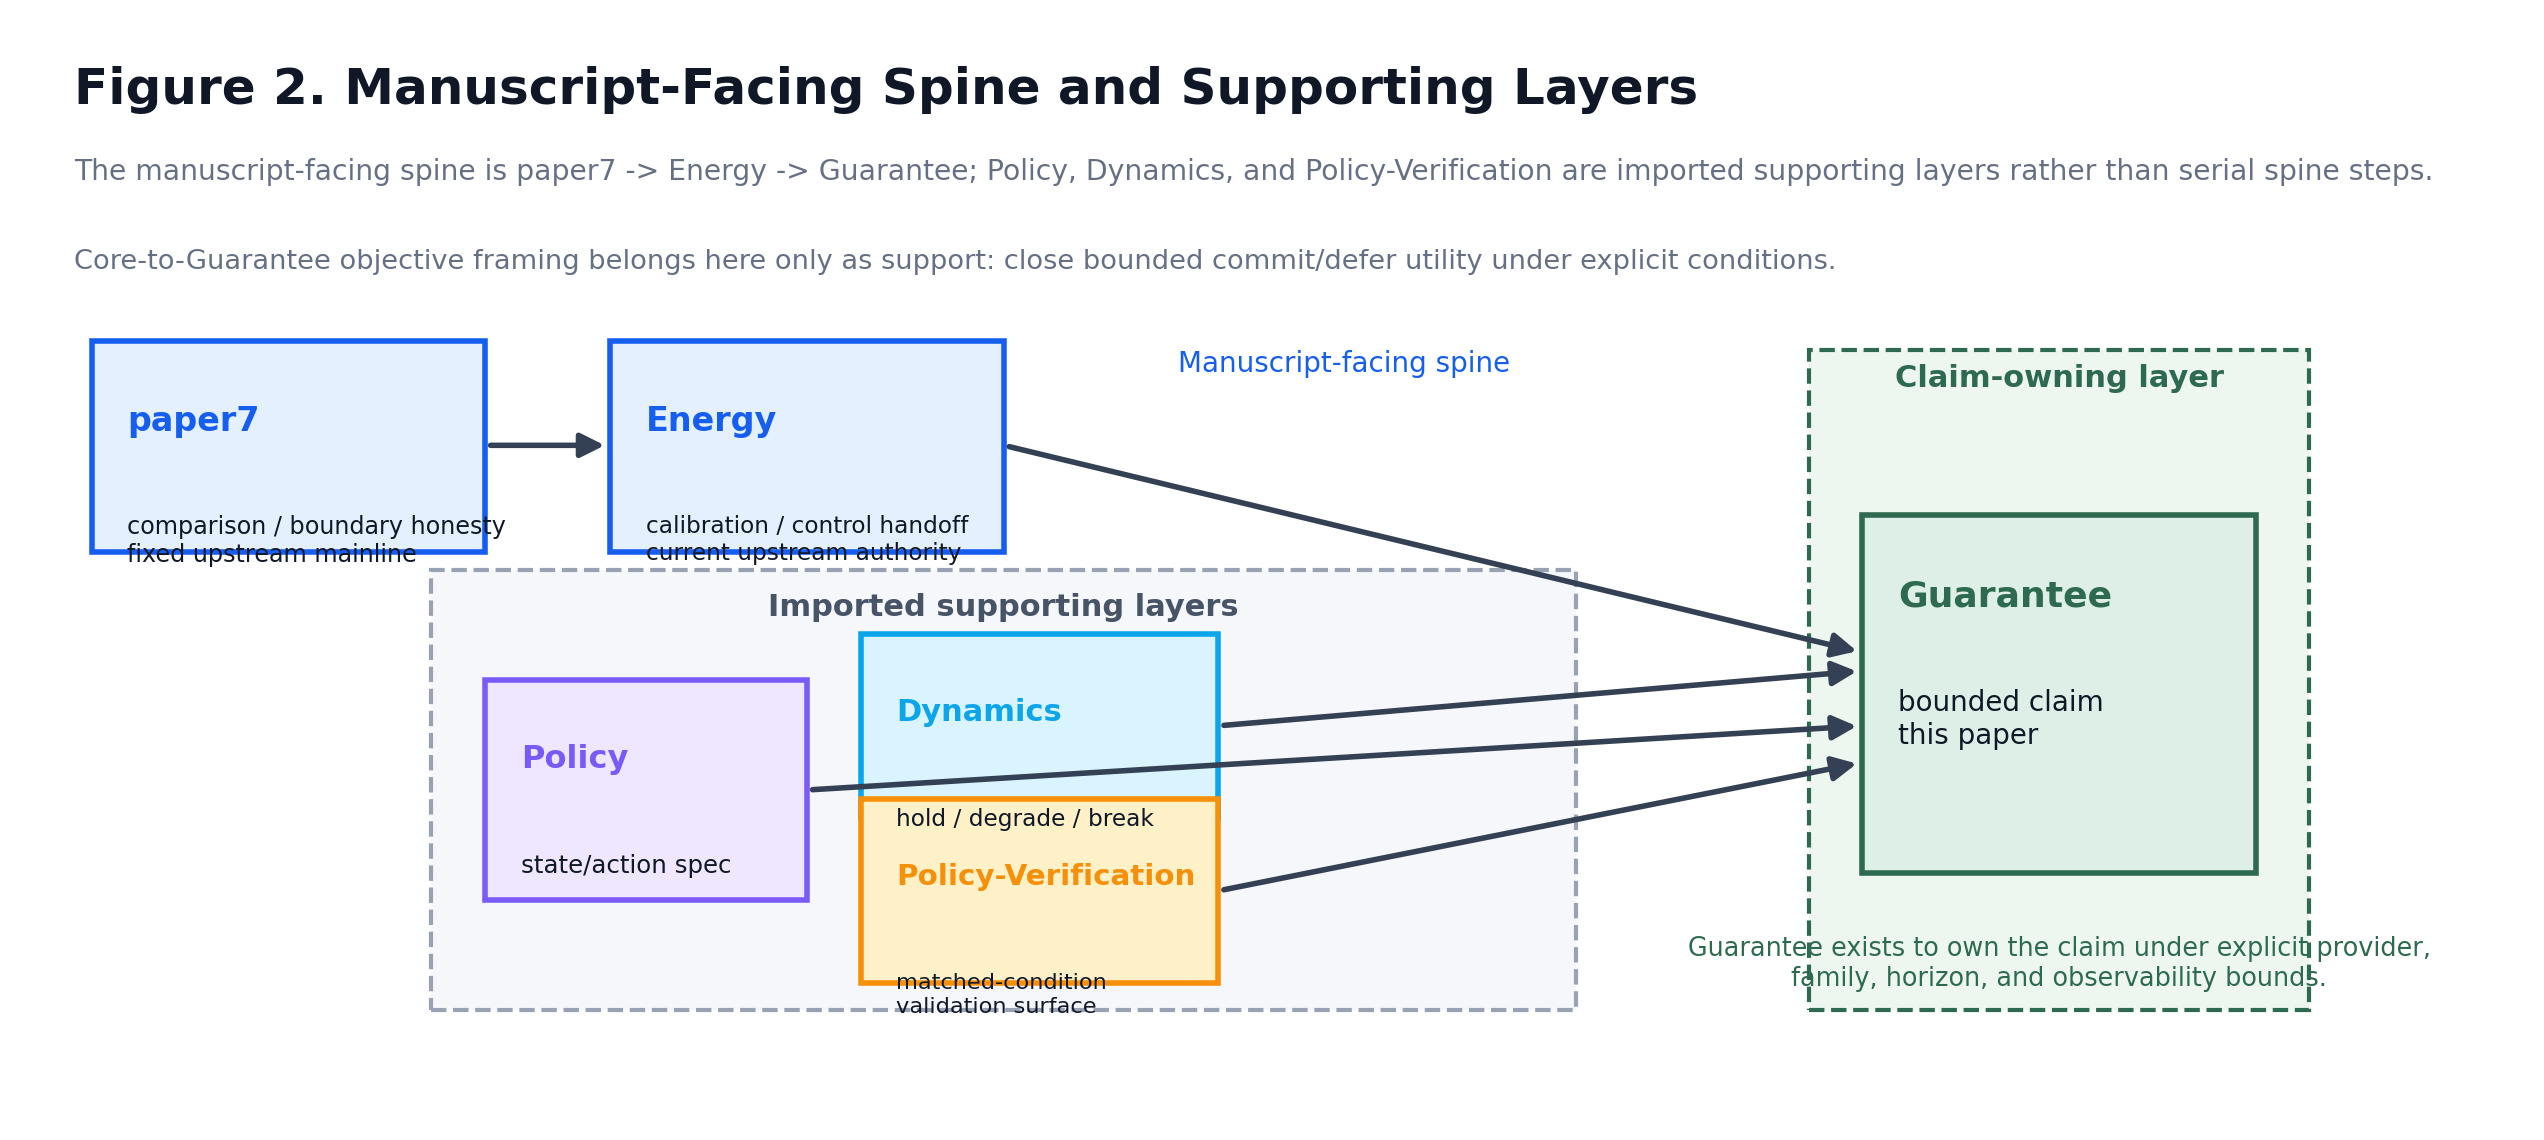
\includegraphics[width=\textwidth]{fig2_guarantee_centered_architecture_v1.png}
\caption{Current manuscript-facing dependency structure.
Integrated \texttt{paper7} and \texttt{Energy} remain the manuscript-facing
upstream spine, while \texttt{Policy}, \texttt{Dynamics}, and
\texttt{Policy-Verification} are imported supporting layers rather than serial
spine steps. \texttt{Guarantee} carries the current bounded supported and
supporting, and boundary surfaces.}
\end{figure}

\section{Supporting-Layer Inputs}

\subsection{Policy Input}

The current policy layer fixes the downstream state vocabulary
(\texttt{active\_objective}, \texttt{suspended\_objective},
\texttt{accepted\_direction}, \texttt{unresolved\_relation},
\texttt{quarantine}, \texttt{local\_relation\_block}) together with the minimal
commit/defer action set. The \texttt{Guarantee} line inherits this vocabulary as
its operating language and does not redesign it locally.

That vocabulary is not ornamental. The early ambiguity-turn surface is the
cleanest current instance of \texttt{defer\_with\_resolution}: no content work
should begin before a direction is accepted, and no unilateral priority choice
should be made on the user's behalf. The downstream acceptance surface is the
current instance of \texttt{commit\_to\_accepted\_direction} in which the
honest carry-forward read is bounded support for
\texttt{preacceptance\_rework\_burden\_absent} under the mainline comparison
contract, with Gemini residuals still visible beyond that shared gain rather
than broad downstream closure. The
repaired first-step side-topic surface is the clearest
first-step instance of \texttt{accepted\_direction} becoming
\texttt{active\_objective} while the prior line is held as
\texttt{suspended\_objective} under \texttt{quarantine}, but in the current
paper it is carried only as a supporting surface because that read depends on a
local repaired comparison rather than on the manuscript's inherited mainline
comparison contract. The later-horizon
boundary then marks the point where \texttt{unresolved\_relation} handling
weakens and \texttt{local\_relation\_block} is no longer treated conservatively.
For the current downstream line, preserving an unresolved relation should also
be read in a narrower but more practical sense than mere recommendation
avoidance. Once a branch has already been accepted, failure can still occur if
the next assistant move silently compresses still-live user-side constraint or
satisfaction structure into one asserted local reading. The manuscript does not
expand that point into a general hidden-needs thesis. It uses it only to mark a
bounded downstream failure mode: advancing as though the user's governing
criterion were already fixed when the visible interaction state does not yet
support that fixation.

\subsection{Dynamics Input}

The current dynamics layer contributes mechanism vocabulary only. Its role is to
name where the inherited policy state holds, weakens, or breaks across later
checkpoints. In the current branch, the key motifs are \textit{Stable
Resolution}, \textit{Clean Quarantine Hold}, \textit{Useful Continuation Hold},
\textit{Relation-Preservation Hold}, \textit{Premature Relation Collapse},
\textit{Repeated-Starter Attractor}, \textit{Generic Stall}, and
\textit{Quarantine Leak}.

Using that vocabulary makes the manuscript read as one bounded progression rather
than as three disconnected pilot wins. The ambiguity-turn result is the clearest
instance of \textit{Stable Resolution}. The repaired first-step side-topic
supporting surface is the clearest instance of \textit{Clean Quarantine Hold}.
The downstream
acceptance result remains narrower: under the manuscript's inherited
\texttt{baseline vs Energy policy} comparison, the shared supported behavior is
bounded removal of \texttt{preacceptance\_rework\_burden\_absent}, but Gemini
\texttt{accepted\_direction\_followthrough\_present} drops from
\texttt{13 / 24} to \texttt{10 / 24}, and the auxiliary repaired
\texttt{NRR vs Ablation} read remains mixed, with Anthropic \texttt{Baseline}
still stronger than Anthropic \texttt{NRR} on \texttt{appropriate}. That
surface should not yet be collapsed into uniform \textit{Useful Continuation
Hold}. Because the repaired side-topic read depends on a local repaired
comparison, it remains supporting evidence rather than a second supported
claim. The later-horizon boundary is best read as weakening
\textit{Relation-Preservation Hold} before \textit{Premature Relation Collapse}
appears, with more local residual forms such as \textit{Generic Stall} or
\textit{Repeated-Starter Attractor} where the template/provider slice warrants
them.

\subsection{Policy-Verification Input}

The current policy-verification layer fixes the protocol rules that any prospective
\texttt{baseline vs Energy policy} comparison must satisfy before guarantee text is
allowed. This includes matched-condition comparison, pre-frozen reporting
surfaces, narrow family selection, explicit horizon bands, and main-text
reporting of both gains and failure boundaries.

\subsection{Experimental Conditions}

The carried surfaces in this manuscript are reported as frozen matched-condition
row totals rather than as claims of independent stochastic sampling. The early
ambiguity-turn pilot uses temperature \texttt{0.0}, three templates, and eight
reps per provider/arm, so each provider slice is reported over \texttt{24}
rows at one early decision boundary. The downstream-acceptance pilot also uses
temperature \texttt{0.0}, the same three templates, and four reps per
acceptance variant across two acceptance variants, again yielding \texttt{24}
rows per provider slice at the first accepted-direction boundary. The repaired
first-step side-topic / quarantine pilot uses temperature \texttt{0.0}, the
same three templates, \texttt{accept\_side\_first} only, and four reps per
provider/arm, yielding \texttt{12} rows per provider slice at \texttt{turn5}.
The later-horizon boundary then reports later checkpoints \texttt{turn7},
\texttt{turn9}, and \texttt{turn11} over \texttt{12} episodes per provider in
a separate frozen \texttt{priority-resolution horizon-stability} family that
reads the later continuation of the carried side-topic line. The numerators
and denominators in the manuscript should therefore be read as fixed-condition
row counts under frozen prompts, models, and templates, not as
provider-universal frequency estimates.

\section{Claim, Supporting-Surface, And Boundary Discipline}

Any supported claim, supporting surface, or explicit boundary surface in this
paper must disclose a bounded reporting surface with the following fields:

\begin{enumerate}
\item provider scope
\item family scope
\item horizon scope
\item observability scope
\item comparison scope
\item supported behavior
\item explicit failure boundary
\item unsupported extension
\end{enumerate}

These fields define a shared disclosure schema, not one uniform evidentiary
contract. Supported claims, supporting surfaces, and matched-condition boundary
surfaces must fill all eight fields explicitly. The later-horizon boundary is
instead carried as a diagnostic one-arm later-checkpoint degradation surface:
it still states provider, family, horizon, observability, comparison, supported
behavior, explicit failure boundary, and unsupported extension, but its
comparison scope is explicitly a diagnostic one-arm later-checkpoint read
rather than a matched-comparison fill, and its supported-behavior field remains
boundary-only rather than an additional supported claim. No carried scientific
surface is valid if the fields required by its evidentiary contract are
omitted. This paper therefore inherits the current schema rule that the claim
surface must be chosen before outcome inspection and must remain narrow enough
to prevent provider-universal, family-universal, or long-horizon overreach.

\begin{table}[ht]
\centering
\begin{tabular}{|p{0.13\textwidth}|p{0.27\textwidth}|p{0.22\textwidth}|p{0.24\textwidth}|}
\hline
\textbf{Unit} & \textbf{Scope} & \textbf{Supported behavior} & \textbf{Boundary kept explicit} \\
\hline
Early ambiguity-turn & Tested provider pair, frozen priority-resolution family, early decision boundary & Non-unilateral priority resolution & No downstream acceptance, side-topic/quarantine, or later-horizon extension \\
\hline
Downstream acceptance boundary & Tested provider pair, downstream-acceptance family, first accepted-direction boundary & Bounded support for preacceptance burden removal under matched baseline vs Energy-policy conditions & Keep Gemini residuals and the auxiliary repaired read explicit; do not collapse into pair-wide or provider-universal downstream-guarantee language \\
\hline
Side-topic/quarantine supporting surface & Tested provider pair, repaired side-topic family, first accepted side-topic workstart checkpoint & Clean first-step side-topic workstart under explicit side-first acceptance on a local repaired comparison & Keep it as supporting evidence only; do not upgrade the local repaired comparison into a second manuscript supported claim or later-horizon stability read \\
\hline
Later-horizon boundary & Tested provider pair, priority-resolution horizon-stability family, later checkpoints \texttt{turn7}/\texttt{turn9}/\texttt{turn11}, diagnostic one-arm later-checkpoint read & Boundary-only read: relation preservation weakens before suspended-main quarantine breaks & Keep later-horizon as diagnostic boundary reporting only; no matched-comparison fill, no fourth supported claim, and no provider-universal or long-horizon extension \\
\hline
\end{tabular}
\caption{Current supported, supporting, and boundary surfaces in
\texttt{Guarantee}.}
\end{table}

\begin{figure}[ht]
\centering
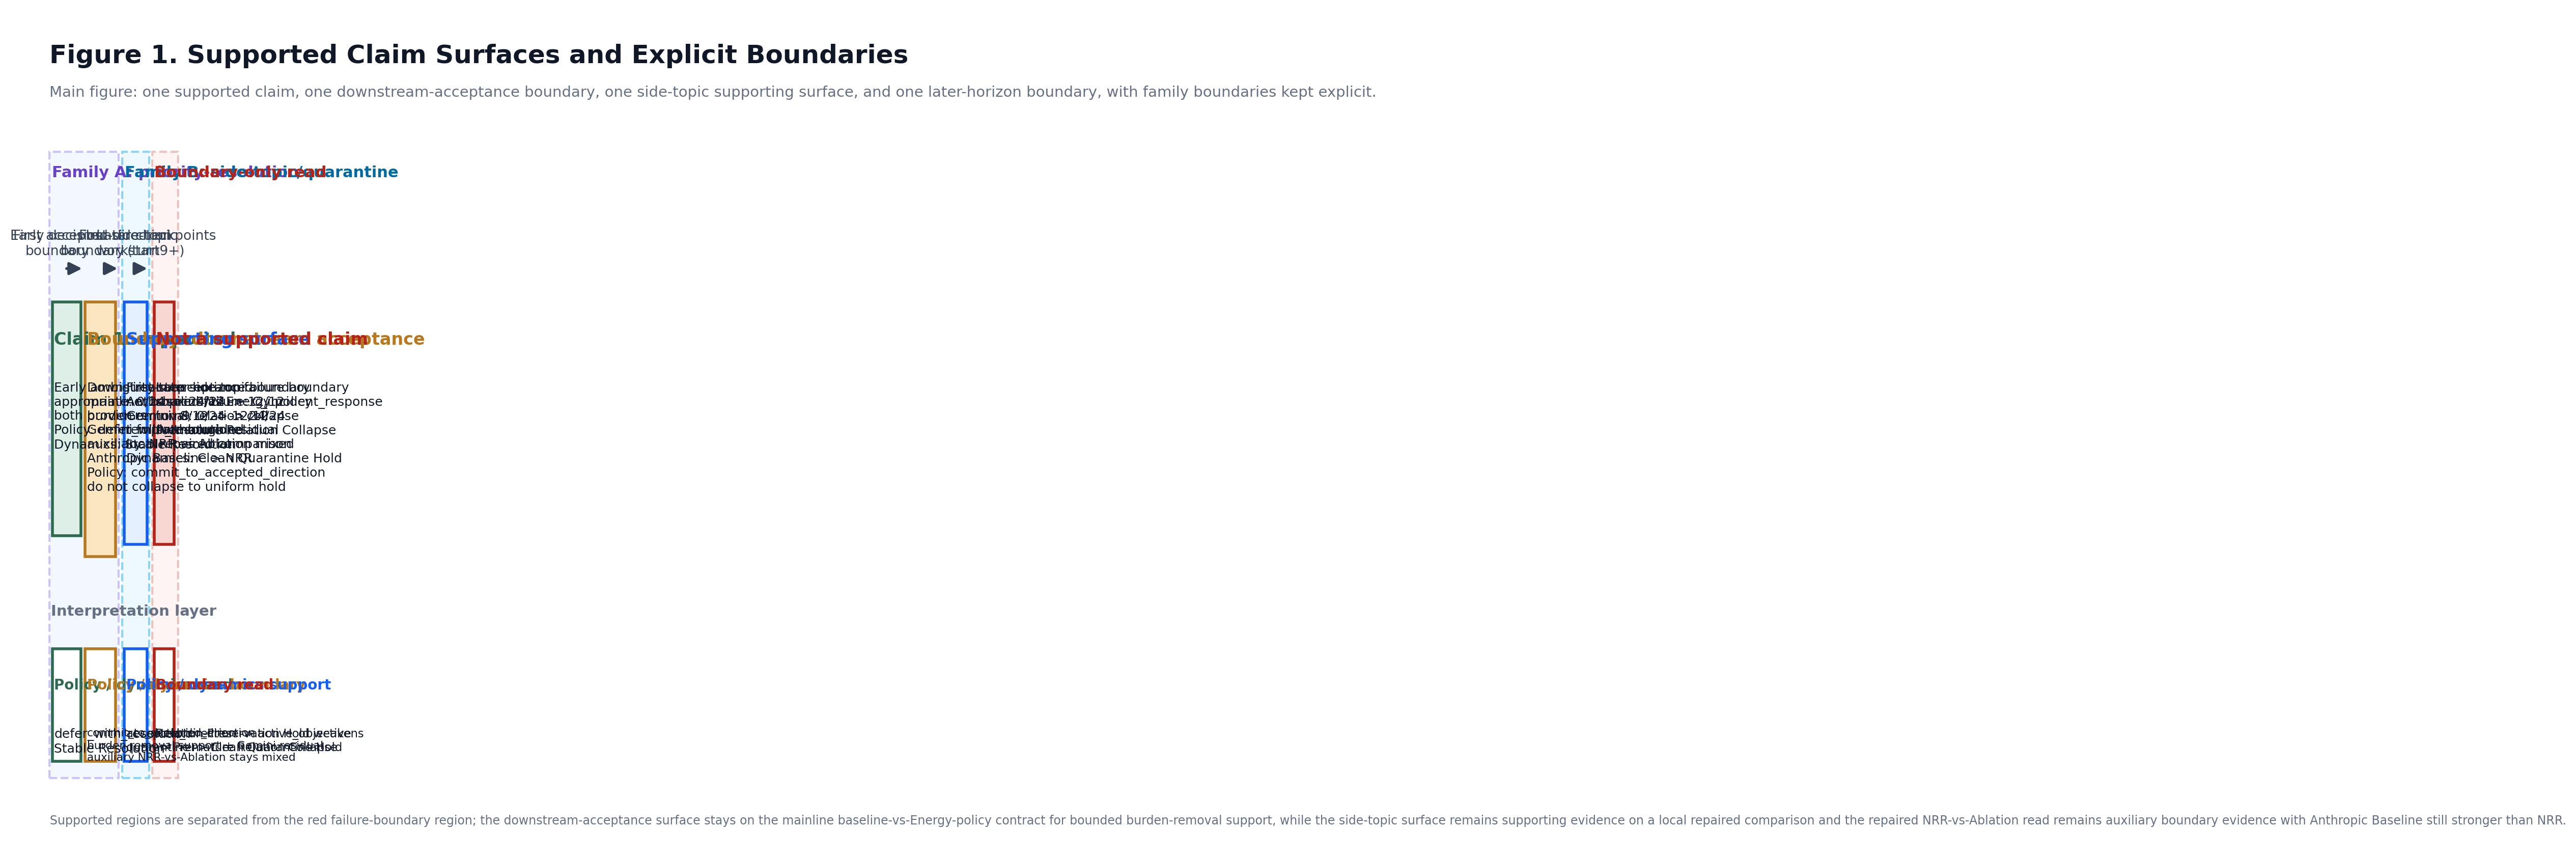
\includegraphics[width=\textwidth]{fig1_supported_claim_progression_v1.png}
\caption{Supported claim progression, supporting evidence, and explicit
boundary surfaces. Claim 1 and the downstream-acceptance boundary occupy
different horizon points within the same \texttt{priority-resolution} family,
while the side-topic/quarantine read belongs to a separate repaired family and
is carried only as supporting evidence. The later-horizon region is a separate
\texttt{priority-resolution horizon-stability} boundary read over the later
continuation of that carried line rather than an additional supported claim.}
\end{figure}

\subsection{First Supported Claim Unit}

The first explicit supported claim unit in the current manuscript is:

\begin{itemize}
\item provider scope:
  the tested provider pair only (\texttt{claude-sonnet-4-6} and
  \texttt{gemini-2.0-flash})
\item family scope:
  the frozen \texttt{priority-resolution} ambiguity-turn family only
\item horizon scope:
  the early decision boundary only
\item observability scope:
  \texttt{resolution\_attempt\_present},
  \texttt{unilateral\_commit\_absent}, and \texttt{appropriate}
\item comparison scope:
  matched baseline vs Energy-policy under the frozen early
  ambiguity-turn pilot conditions
\item supported behavior:
  non-unilateral priority resolution
\item explicit failure boundary:
  no downstream acceptance, side-topic/quarantine, or later-horizon closure is
  established by this fill
\item unsupported extension:
  no provider-universal, long-horizon, or broad downstream-quality claim is
  authorized
\end{itemize}

In manuscript form, the bounded claim is:

\begin{quote}
Under the tested provider pair, for the frozen \texttt{priority-resolution}
ambiguity-turn family, at the early decision boundary, and on the directly scored
fields \texttt{resolution\_attempt\_present},
\texttt{unilateral\_commit\_absent}, and \texttt{appropriate}, the Energy-policy
arm is supported relative to matched baseline only for non-unilateral priority
resolution. This support excludes downstream acceptance, side-topic/quarantine,
and later-horizon behavior, and it does not extend to provider-universal or broad
downstream-quality claims.
\end{quote}

\subsection{Downstream-Acceptance Boundary Surface}

The current downstream-acceptance boundary surface in the manuscript is:

\begin{itemize}
\item provider scope:
  the tested provider pair only (\texttt{claude-sonnet-4-6} and
  \texttt{gemini-2.0-flash})
\item family scope:
  the downstream-acceptance family only
\item horizon scope:
  the first accepted-direction downstream boundary only
\item observability scope:
  \texttt{accepted\_direction\_followthrough\_present},
  \texttt{rejected\_direction\_intrusion\_absent},
  \texttt{preacceptance\_rework\_burden\_absent}, and \texttt{appropriate}
\item comparison scope:
  matched baseline vs Energy-policy under the frozen downstream-boundary pilot
  conditions, with reviewed \texttt{NRR vs Ablation} retained only as an
  auxiliary repaired boundary comparator
\item supported behavior:
  bounded support for removal of preacceptance rework burden under the first
  accepted-direction downstream boundary
\item explicit failure boundary:
  the surface does not close as pair-wide downstream quality, provider-universal
  continuation support, explicit quarantine closure, or later-horizon
  continuation stability; Gemini
  \texttt{accepted\_direction\_followthrough\_present} drops from
  \texttt{13 / 24} to \texttt{10 / 24}, and the auxiliary repaired read
  remains mixed
\item unsupported extension:
  no pair-wide downstream-acceptance guarantee, explicit quarantine closure, or
  later-horizon stability claim is authorized, and no manuscript claim that the
  auxiliary repaired \texttt{NRR vs Ablation} read replaces the paper-level
  comparison contract
\end{itemize}

In manuscript form, the bounded boundary read is:

\begin{quote}
Under the tested provider pair, for the downstream-acceptance family, at the
first accepted-direction downstream boundary, and on the directly scored fields
\texttt{accepted\_direction\_followthrough\_present},
\texttt{rejected\_direction\_intrusion\_absent},
\texttt{preacceptance\_rework\_burden\_absent}, and \texttt{appropriate}, the
matched \texttt{baseline vs Energy policy} surface supports only bounded
removal of preacceptance rework burden rather than pair-wide downstream-quality
closure: both provider slices reach \texttt{24 / 24} on
\texttt{preacceptance\_rework\_burden\_absent}, but Gemini
\texttt{accepted\_direction\_followthrough\_present} simultaneously drops from
\texttt{13 / 24} to \texttt{10 / 24} on the same mainline comparison surface.
The
reviewed \texttt{NRR vs Ablation} read remains auxiliary boundary evidence
only: Gemini reaches support there, Anthropic remains inconclusive, and the
Anthropic-side auxiliary comparison keeps \texttt{Baseline} stronger than
\texttt{NRR} on \texttt{appropriate}. This surface is therefore carried forward
only as a bounded downstream-boundary result, not as a pair-wide downstream
guarantee, explicit quarantine closure, or later-horizon stability claim.
\end{quote}

The auxiliary repaired read uses a narrower direct trace than the mainline
protocol-era fields: \texttt{accepted\_branch\_followthrough\_present} maps to
\texttt{accepted\_direction\_followthrough\_present},
\texttt{reopened\_choice\_absent} plus
\texttt{alternative\_branch\_push\_absent} jointly trace the manuscript's
rejected-direction non-intrusion requirement, and that mapping is kept explicit
in the bundled closure import note rather than treated as a one-to-one field
replacement.

\subsection{Side-Topic / Quarantine Supporting Surface}

Because this surface depends on a local repaired
\texttt{baseline vs revised Energy policy} comparison rather than on the
paper-level mainline \texttt{baseline vs Energy policy} contract, it is carried
here as a bounded supporting surface and not as a second manuscript supported
claim unit.

The repaired first-step side-topic / quarantine supporting surface in the
current manuscript is:

\begin{itemize}
\item provider scope:
  the tested provider pair only (\texttt{claude-sonnet-4-6} and
  \texttt{gemini-2.0-flash})
\item family scope:
  the repaired first-step side-topic / quarantine family only
\item horizon scope:
  the first accepted side-topic workstart checkpoint only
\item observability scope:
  \texttt{chosen\_side\_direction\_workstart\_present},
  \texttt{suspended\_main\_reference\_absent},
  \texttt{main\_direction\_intrusion\_absent}, and \texttt{appropriate}
\item comparison scope:
  matched baseline vs revised Energy-policy under the repaired first-step
  side-topic / quarantine pilot conditions
\item supported behavior:
  clean first-step side-topic workstart under explicit side-first acceptance
\item explicit failure boundary:
  the gain is incremental rather than a rescue from total baseline failure, and
  the main lift over baseline is concentrated in \texttt{C\_incident\_response};
  because this read uses a local repaired comparison rather than the inherited
  paper-level contract, it is carried as supporting evidence rather than as a
  manuscript supported claim unit
\item unsupported extension:
  no provider-universal side-topic commitment, uniform template lift, later-
  horizon side-topic stability claim, or upgrade to a second manuscript
  supported claim is authorized
\end{itemize}

In manuscript form, the bounded supporting read is:

\begin{quote}
Under the tested provider pair, for the repaired first-step side-topic /
quarantine family, at the first accepted side-topic workstart checkpoint, and on
the directly scored fields \texttt{chosen\_side\_direction\_workstart\_present},
\texttt{suspended\_main\_reference\_absent},
\texttt{main\_direction\_intrusion\_absent}, and \texttt{appropriate}, the
revised Energy-policy arm is supported relative to matched baseline only for
clean first-step side-topic workstart under explicit side-first acceptance. This
surface is carried only as bounded supporting evidence because its comparison
contract is the repaired local \texttt{baseline vs revised Energy policy}
surface rather than the manuscript's mainline \texttt{baseline vs Energy
policy} contract. It excludes provider-universal side-topic commitment,
uniform template lift, and later-horizon side-topic stability, and it remains
bounded by the fact that the main incremental lift over baseline is
concentrated in \texttt{C\_incident\_response}.
\end{quote}

\section{Evidence Import Surface}

The scientific argument in this manuscript draws on three bundled evidence
layers. Fixed supporting-layer texts provide the inherited program-design,
policy, dynamics, protocol, and historical handoff vocabulary that is imported
without reopening ownership locally. Repo-local analysis notes then fix the
current manuscript-facing reads for the early ambiguity-turn claim, the
downstream-acceptance boundary, the repaired first-step side-topic /
quarantine supporting surface, the later-horizon boundary, the
policy/dynamics interpretation layer, and the current upstream spine
interpretation. An imported reviewed readout surface preserves the repaired
\texttt{NRR vs Ablation} downstream comparison as auxiliary boundary evidence
only.

Detailed artifact routing, filenames, and review-package entrypoints are kept
outside the scientific body in \texttt{reproducibility.md} and the current
supporting-layer evidence map. The manuscript body uses those bundled inputs to
state the bounded scientific read rather than to reproduce the repository
manifest inline.

This split is deliberate. The support bundle carries fixed upstream dependency
texts and historical provenance; it is not by itself the manuscript-facing
proof surface for every later bounded surface. In particular, the older downstream-
acceptance memo preserved in \texttt{supporting\_layer\_sources/current/}
remains a pre-repair historical read. The current downstream-acceptance
boundary surface is instead anchored by the repo-local closure import note, the
repo-local boundary-surface note, the directly shipped baseline-vs-Energy
comparison memo with its four run-annotation CSVs, and the imported reviewed
auxiliary repaired surface listed above. The shipped bundle now also includes
the repaired side-topic comparison memo together with its four run-annotation
CSVs, and the later-horizon two-provider memo together with the provider-scored
read memos and run-annotation CSVs needed to inspect that boundary one layer
below the manuscript-facing drafting memos.

\subsection{First Evidence Import}

The strongest current entry point for the \texttt{Guarantee} line is the frozen
early ambiguity-turn pilot. Under matched baseline vs Energy-policy conditions,
both tested provider slices moved from \texttt{0 / 24} to \texttt{24 / 24} on
\texttt{resolution\_attempt\_present}, from \texttt{8 / 24} to
\texttt{24 / 24} on \texttt{unilateral\_commit\_absent}, and from
\texttt{0 / 24} to \texttt{24 / 24} on \texttt{appropriate}. Baseline failure
modes remained visible as either ambiguity-preserving but unresolved responses
or unilateral/content-before-resolution behavior. The carry-forward read is
therefore that the Energy-policy surface supports
non-unilateral priority resolution at the early decision boundary on the tested
provider pair. This is a bounded early-control claim only; it does not by
itself establish downstream followthrough, quarantine behavior,
later-horizon stability, or provider-universal validity.

\subsection{Second Evidence Import}

The downstream-acceptance boundary is the current second \texttt{Guarantee}
entry point. The inherited paper-level comparison contract stays on matched
\texttt{baseline vs Energy policy} conditions, where both tested provider
slices move from \texttt{0 / 24} to \texttt{24 / 24} on
\texttt{preacceptance\_rework\_burden\_absent}. That shared gain is the current
supported downstream-boundary behavior. The residual remains visible in the
same mainline surface: Gemini still shows partial first accepted-direction
followthrough on part of the tested rows, so the claim does not close as
pair-wide downstream-quality support. The imported reviewed readout then keeps a
narrower auxiliary repaired comparison visible directly inside this repository:
on reviewed \texttt{NRR vs Ablation}, Gemini reaches support, Anthropic remains
inconclusive, and the same reviewed memo keeps Anthropic \texttt{Baseline}
stronger than Anthropic \texttt{NRR} on \texttt{appropriate}. The truthful
carry-forward read is therefore bounded support for preacceptance burden
removal under the mainline comparison, with the repaired \texttt{NRR vs
Ablation} surface used only as auxiliary boundary evidence. This surface does
not yet license pair-wide downstream guarantee language, explicit quarantine
closure, later-horizon stability claims, or any claim that the auxiliary
repaired read replaces the paper-level comparison contract.

\subsection{Third Evidence Import}

The third manuscript-facing \texttt{Guarantee} entry point is the repaired
first-step side-topic / quarantine supporting surface. Under matched baseline
vs revised Energy-policy conditions, the revised arm reached
\texttt{appropriate = 12 / 12} in both provider slices, but the honest read is
incremental rather than global: baseline was already fairly strong on
\texttt{A\_trip\_planning} and \texttt{B\_hiring\_packet}, and the main lift
over baseline concentrated in \texttt{C\_incident\_response}
(\texttt{1 / 4 -> 4 / 4} on Anthropic and \texttt{0 / 4 -> 4 / 4} on Gemini).
Because this surface sits on a local repaired
\texttt{baseline vs revised Energy policy} comparison rather than on the
paper-level mainline contract, the carry-forward read is a bounded
first-step side-topic workstart supporting surface under explicit side-first
acceptance, not a second manuscript supported claim and not a universal
side-topic/quarantine or later-horizon stability claim.

\paragraph{Behavior-First Manipulation Check}

A separate provider-pair rerun on the repaired behavior-first surface does not
enter this paper as a supported \texttt{Guarantee} claim unit or as a boundary
surface. Its narrower
manuscript role is to show that, on the tested provider pair, repaired
opening-comparison insertion produces a readable change in first-move behavior:
implementation responses mostly remained in direct relation work, whereas
ablation responses mostly opened with comparison-heavy framing. This result is
therefore carried here only as bounded behavioral-separation evidence. It does
not establish a clean two-stage realization: the ablation arm still most often
opens with comparison framing and then continues with a follow-up question
rather than separating those moves cleanly, Anthropic \texttt{D2} remains a
\texttt{1 / 10} collapse row, and the rerun does not establish pair-level
continuation-quality superiority. Its role in this manuscript is therefore a
secondary bounded note inside the evidence-import discussion rather than a main
claim unit or boundary surface.

\paragraph{Formal Carried Surfaces}

The formal scientific surfaces carried by this manuscript are therefore three
comparison-backed carried surfaces plus one diagnostic later-horizon boundary:
\begin{itemize}
\item Early ambiguity-turn supported claim: tested provider pair, early
decision boundary, and direct observability on
\texttt{resolution\_attempt\_present}, \texttt{unilateral\_commit\_absent}, and
\texttt{appropriate}.
\item Downstream-acceptance boundary: tested provider pair, first accepted-
direction downstream boundary, and direct observability on
\texttt{accepted\_direction\_followthrough\_present},
\texttt{rejected\_direction\_intrusion\_absent},
\texttt{preacceptance\_rework\_burden\_absent}, and \texttt{appropriate}.
\item First-step side-topic / quarantine supporting surface: tested provider
pair, first accepted side-topic workstart checkpoint, and direct observability on
\texttt{chosen\_side\_direction\_workstart\_present},
\texttt{suspended\_main\_reference\_absent},
\texttt{main\_direction\_intrusion\_absent}, and \texttt{appropriate}; this
surface remains supporting evidence because it depends on a local repaired
\texttt{baseline vs revised Energy policy} comparison.
\item Later-horizon failure boundary: tested provider pair, measured later
  checkpoints especially \texttt{turn9}, and relation-preservation failure
  surfaces under a diagnostic one-arm later-checkpoint read.
\end{itemize}

The behavior-first rerun remains outside this formal surface list and is
carried only as a secondary bounded behavioral-separation note.

\subsection{Policy/Dynamics Interpretation Layer}

Taken together, these carried surfaces define a bounded progression rather than
a universal recipe. They share one disclosure schema, but not one uniform
evidentiary contract: the first three surfaces are comparison-backed, while the
later-horizon boundary is a diagnostic later-checkpoint read. At the earliest
boundary, the supported behavior is
\texttt{defer\_with\_resolution} and the corresponding dynamics motif is
\textit{Stable Resolution}. At the downstream acceptance boundary, the
supported behavior is bounded burden removal under matched \texttt{baseline vs
Energy policy} conditions, but Gemini still retains first-followthrough
residuals and the auxiliary repaired \texttt{NRR vs Ablation} read remains
mixed, so this surface cannot yet be read as pair-wide \textit{Useful
Continuation Hold}. At the repaired first-step side-topic supporting surface,
the carried behavior is a clean transition from
\texttt{accepted\_direction} into \texttt{active\_objective} with
\texttt{suspended\_objective} still held in quarantine, which corresponds to
\textit{Clean Quarantine Hold}. Because that surface depends on a local
repaired comparison, it remains supporting evidence rather than the paper's
second supported claim. The later-horizon limit then becomes easier to state
precisely: the first broad break is not simple suspended-main reactivation but
weakening \textit{Relation-Preservation Hold} until \textit{Premature
Relation Collapse} appears.

\begin{table}[ht]
\centering
\begin{tabular}{|p{0.18\textwidth}|p{0.22\textwidth}|p{0.22\textwidth}|p{0.2\textwidth}|}
\hline
\textbf{Surface} & \textbf{Anthropic-side read} & \textbf{Gemini-side read} & \textbf{Boundary implication} \\
\hline
Early ambiguity-turn & Clean support on the tested early surface & Clean support on the tested early surface & Safe to state only a bounded early-control claim, not broader downstream closure \\
\hline
Downstream acceptance boundary & Mainline burden-removal support is clean; auxiliary repaired read stays \texttt{inconclusive} and keeps \texttt{Baseline} stronger than \texttt{NRR} on \texttt{appropriate} & Mainline burden-removal support is present, but \texttt{accepted\_direction\_followthrough\_present} drops from \texttt{13 / 24} to \texttt{10 / 24}; auxiliary repaired read reaches \texttt{support} & Keep the claim at bounded burden-removal support under the mainline contract; use the repaired read only as boundary evidence, not as a replacement comparison rule \\
\hline
First-step side-topic / quarantine & Lift is visible, with strongest incremental gain on \texttt{C\_incident\_response} & Lift is also visible, again with the main gain concentrated on \texttt{C\_incident\_response} & Treat the result as template-bounded improvement, not uniform side-topic stability \\
\hline
Later-horizon boundary & Degradation remains visible at later checkpoints & Degradation remains visible at later checkpoints & Preserve later-horizon text as boundary reporting rather than a fourth supported guarantee \\
\hline
\end{tabular}
\caption{Provider-specific residual structure that keeps the current
\texttt{Guarantee} claims bounded.}
\end{table}

\section{Later-Horizon Failure Boundary}

The current later-horizon boundary surface in the manuscript is:

\begin{itemize}
\item provider scope:
  the tested provider pair only (\texttt{claude-sonnet-4-6} and
  \texttt{gemini-2.0-flash})
\item family scope:
  the frozen \texttt{priority-resolution horizon-stability} family only,
  separate from the repaired first-step side-topic/quarantine family and used
  to read the later continuation of the carried side-topic line
\item horizon scope:
  later checkpoints \texttt{turn7}, \texttt{turn9}, and \texttt{turn11} only,
  with \texttt{turn9} the first shared clean failure checkpoint
\item observability scope:
  \texttt{chosen\_side\_direction\_progress\_present},
  \texttt{user\_detail\_use\_present},
  \texttt{unresolved\_relation\_preserved\_or\_narrowly\_checked},
  \texttt{suspended\_main\_reference\_absent},
  \texttt{starter\_question\_repeat\_absent}, and \texttt{appropriate}
\item comparison scope:
  not a matched comparison fill; diagnostic one-arm later-checkpoint read over
  the provider-scored annotation tables for the active later-horizon family
\item supported behavior:
  boundary-only detection that relation preservation weakens before suspended-
  main quarantine breaks, with the limited safe hold that the first side-topic
  switch can survive into the next checkpoint
\item explicit failure boundary:
  later degradation remains real, template-dependent, and provider-sensitive;
  the clearest shared failure surface is \texttt{C\_incident\_response} at
  \texttt{turn9}, where both providers collapse the unresolved relation by
  prematurely committing an ordering between \texttt{impact} and
  \texttt{root cause}
\item unsupported extension:
  no matched-comparison claim, no fourth supported \texttt{Guarantee} claim,
  no provider-universal or family-universal degradation depth, no long-horizon
  stability guarantee, and no claim that prompt-layer control alone secures
  stable \texttt{turn11} behavior
\end{itemize}

In manuscript form, the bounded later-horizon boundary read is:

\begin{quote}
Under the tested provider pair, for the frozen
\texttt{priority-resolution horizon-stability} family, kept separate from the
repaired first-step side-topic/quarantine family but used to read the later
continuation of the carried side-topic line, at later checkpoints
\texttt{turn7}, \texttt{turn9}, and \texttt{turn11}, and on the directly scored
fields \texttt{chosen\_side\_direction\_progress\_present},
\texttt{user\_detail\_use\_present},
\texttt{unresolved\_relation\_preserved\_or\_narrowly\_checked},
\texttt{suspended\_main\_reference\_absent},
\texttt{starter\_question\_repeat\_absent}, and \texttt{appropriate}, the
current later-horizon surface is carried only as a diagnostic one-arm boundary
read, not as a matched-comparison fill. The limited safe hold is that the
first side-topic switch can survive into the next checkpoint while suspended-
main quarantine remains visible, but later degradation remains real,
template-dependent, and provider-sensitive. The clearest shared failure surface
is \texttt{C\_incident\_response} at \texttt{turn9}, where both providers
collapse the still unresolved relation by prematurely committing an ordering
between \texttt{impact} and \texttt{root cause}. The correct read is therefore
that later-horizon instability emerges through weakening relation preservation
before suspended-main quarantine itself breaks. This later-horizon material is
a boundary on the current supported surfaces only: it does not authorize a
matched-comparison claim, a fourth supported \texttt{Guarantee} claim,
provider-universal degradation depth, or long-horizon stability language.
\end{quote}

\section{Reproducibility And Repository Surface}

The tracked repository surface for this manuscript is intentionally narrow and
repo-local:
\begin{itemize}
\item a current TeX source
\item a current PDF snapshot
\item the current figure assets used by that TeX source
\item a working drafting outline
\item a supporting-layer evidence map
\item bounded claim, supporting-surface, and boundary drafting memos
\item an imported reviewed downstream-acceptance readout surface for the
current downstream boundary
\item a secondary behavior-first manipulation-check note
\item a later-horizon failure-boundary memo
\item a policy/dynamics manuscript-integration memo
\item a bundled supporting-layer source surface
\item stable build and verification wrappers
\end{itemize}

The repository therefore exposes both the manuscript-facing claim surface and
the specific imported source layers used to justify it. Checksum verification
executes on the tracked current artifact set, and the documented build wrapper
produces a current PDF in this environment through a source-rendered fallback
when cached TeX resources are incomplete. Full typeset reproduction therefore
remains environment-dependent here, but the tracked repository surface is
organized so the bounded claim surface, its imported reviewed downstream-
boundary readout, and its support sources can be inspected without workspace-
only links. Stripped comparison bundles are not the same thing as this tracked
repository surface.

\section{Discussion}

The non-evaluative principle should enter this line as bounded engineering
discipline rather than theorem inflation. In the current read, the practical issue
is not simply whether unresolved content exists, but whether later interaction
forces premature relation collapse while the interaction is still in a retained
state. The \texttt{Guarantee} paper is the correct place to express that read as
a bounded downstream claim surface. In that sense, the manuscript is adjacent to
prior mixed-initiative, clarification, and grounding work, but its objective is
different: it does not primarily propose a better question-asking heuristic or a
general dialogue-success policy. Instead, it asks which bounded commit/defer
claims remain supportable under explicit provider, family, horizon, and
observability restrictions~\cite{chucarroll2000mimic,deboni2003clarification,rao2018evpi,benotti2021grounding,sahay-etal-2025-ask,wen-etal-2025-know,madhusudhan-etal-2025-llms}.

That downstream read should not be reduced to a simple rule of "never recommend
one next move." A response may advance with a provisional recommendation and
still preserve the user's live context if the governing constraint structure
remains visible or explicitly marked as contingent. The harder failure is
premature interpretation fixation: proceeding as if one local reading of the
user's still-live objective, satisfaction condition, or constraint ordering had
already been settled. Framed that way, unresolved-relation preservation is not
mere hesitation. It is bounded context retention under a visible interaction
state.

The current manuscript line also remains deliberately narrow. It is based on
two tested provider slices, one supported early-control claim, one explicit
downstream boundary, one side-topic supporting surface, and one later-horizon
boundary read rather than on a broad cross-provider or long-horizon guarantee.
Those limits are not defects to be hidden: they are part of the bounded-claim
discipline that keeps the manuscript from overstating what the current evidence
surface can support.

This staging matters for how the current line should be read. The manuscript is
not claiming a monotone march from early control support to pair-wide
downstream success. The truthful sequence is narrower: the early ambiguity-turn
surface is clean on the tested provider pair, while the repaired downstream-
acceptance boundary supports only bounded preacceptance-burden removal under
matched \texttt{baseline vs Energy policy} conditions, while Gemini still
shows \texttt{accepted\_direction\_followthrough\_present} dropping from
\texttt{13 / 24} to \texttt{10 / 24} and the auxiliary repaired
\texttt{NRR vs Ablation} read remains mixed, with Anthropic still
\texttt{inconclusive}, Gemini reaching \texttt{support}, and Anthropic
\texttt{Baseline} remaining stronger than Anthropic \texttt{NRR} on
\texttt{appropriate}. On that auxiliary repaired surface, the Anthropic gap is
large rather than cosmetic: \texttt{Baseline} reaches \texttt{142 / 144} on
\texttt{appropriate}, whereas \texttt{NRR} reaches \texttt{55 / 144}. That
auxiliary asymmetry should remain visible because it marks a boundary on the
repaired comparison surface, not because it upgrades the paper-level read. The
paper-level downstream interpretation remains carried by the matched
\texttt{baseline vs Energy policy} surface only: bounded support for
preacceptance-burden removal is visible there, while pair-wide downstream-
quality closure is not. Accordingly, the auxiliary repaired read is kept as
boundary evidence of unresolved downstream fragility rather than as the
authorizing basis for a paper-level early-control / downstream-quality trade-off
claim.

The repaired behavior-first rerun sharpens that boundedness rather than
relaxing it. Its correct manuscript role is a secondary manipulation-check note
inside the evidence-import discussion: it shows that opening-comparison
insertion changes how the next move is framed on the tested provider pair. But
that empirical separation should not be overread as a broader downstream-
quality result. The manipulated form remains compressed, one clear collapse row
remains visible, and the current evidence still falls short of pair-level
continuation-quality superiority. Keeping that limitation adjacent to the
reported rerun result is part of the same bounded-claim discipline rather than
an afterthought.

The present line should also be read as a reusable test surface rather than as
the last word on guarantee behavior. What is fixed here is not an exhaustive
operator set or a closed theorem, but a bounded way to keep later work honest:
explicit supported claims, explicit supporting surfaces, explicit boundary
surfaces, explicit comparison surfaces, provider-sliced reporting, and visible
failure boundaries. That
structure is meant to make follow-on work easier. Later readers should be able
to rerun these guarantee questions under new providers, new downstream
families, new operator variants, and longer horizons without having to guess
which comparison contract or boundary rule the current manuscript relied on.

\section{Conclusion}

This version establishes a bounded manuscript surface for \texttt{Guarantee}.
It carries one supported claim unit for the early ambiguity-turn surface,
carries the downstream-acceptance result forward as an explicit boundary
surface with bounded support for
\texttt{preacceptance\_rework\_burden\_absent} on the mainline
\texttt{baseline vs Energy policy} comparison while keeping the repaired
\texttt{NRR vs Ablation} read as an auxiliary comparator, carries the repaired
first-step side-topic/quarantine result only as a bounded supporting surface
under matched \texttt{baseline vs revised Energy policy} conditions, and keeps
the later-horizon limit explicit as failure-boundary reporting rather than as
a further supported claim. It also ties those supported and unsupported regions
directly to the inherited policy vocabulary and dynamics motifs without
promoting the line into provider-universal, family-universal, or theorem-level
language. In that sense, the present \texttt{Guarantee} line is closer to a
bounded verification/assurance surface over explicit observables than to a
universal correctness claim~\cite{seshia2022verifiedai,desai2019soter}. In
practical terms, the current \texttt{Guarantee} line closes this
pass around a staged bounded result: early control support does not
automatically extend into pair-wide downstream acceptance, the repaired
downstream boundary remains limited to burden removal rather than pair-wide
downstream quality, and the Anthropic-side auxiliary comparison keeps
\texttt{Baseline} stronger than \texttt{NRR} on \texttt{appropriate}. What
remains outside the present claim
surface is broader provider coverage, broader downstream family coverage, and
later-horizon closure. The manuscript therefore aims to do one more thing than
simply close the current bounded read: it fixes a reusable test surface that
later readers can rerun, challenge, and extend under new conditions rather
than treating the present line as exhaustive.

\begin{thebibliography}{99}
\raggedright

\bibitem{saito2025nrr}
K.~Saito,
\newblock ``NRR-Core: Non-Resolution Reasoning as a Computational Framework for Contextual Identity and Ambiguity Preservation,''
\newblock \emph{arXiv preprint arXiv:2512.13478}, 2025.

\bibitem{saito2026phi}
K.~Saito,
\newblock ``NRR-Phi: Text-to-State Mapping for Ambiguity Preservation in LLM Inference,''
\newblock \emph{arXiv preprint arXiv:2601.19933}, 2026.

\bibitem{saito2026ime}
K.~Saito,
\newblock ``NRR-IME: Interface Decomposition for Stable State Transitions on Stateless LLM APIs,''
\newblock GitHub repository: \texttt{https://github.com/kei-saito-research/nrr-ime}; local manuscript snapshot \texttt{paper4-nrr-ime-v67.tex}, commit \texttt{99f5ebb}, 2026.

\bibitem{saito2026transfer}
K.~Saito,
\newblock ``Cross-Task Parser/Update Reuse of a Fixed Hidden-State Operator-Target Interface on Stateless LLM APIs,''
\newblock Series-path repository tree snapshot cited for context only. Manuscript snapshot in cited tree:
\texttt{manuscript/current/paper5-nrr-transfer-v123.tex}. \texttt{https://github.com/kei-saito-research/hidden-state-interface-reuse/tree/24bd24ea183f282cf535205ca4447e8169bac3b0}.

\bibitem{saito2026coupled}
K.~Saito,
\newblock ``NRR-Coupled (cp): Dependency-Consistency Evaluation for Coupled State Updates,''
\newblock Series-path repository tree snapshot cited for context only. Manuscript snapshot in cited tree:
\texttt{manuscript/current/paper6-nrr-coupled-v21.tex}.
\texttt{https://github.com/kei-saito-research/nrr-coupled/tree/aab7cc500acc413d4f585c8a50a9045cb5477eb5}.

\bibitem{saito2026principles}
K.~Saito,
\newblock ``NRR-Patterns: Condition-Bounded Comparison of Five Delayed-Commitment Patterns in Stateful LLM Systems,''
\newblock GitHub repository: \texttt{https://github.com/kei-saito-research/nrr-principles}; bundled authority copy in the active review surface \texttt{supporting\_layer\_sources/current/paper7\_integrated\_manuscript\_v0\_29\_2026-04-01.tex}, 2026.

\bibitem{saito2026energy}
K.~Saito,
\newblock ``NRR-Energy: Calibration of Commit/Defer Utility Under Existing Paired Inputs,''
\newblock GitHub repository: \texttt{https://github.com/kei-saito-research/nrr-energy}; bundled authority copy in the active review surface \texttt{supporting\_layer\_sources/current/nrr-energy\_manuscript\_v26.tex}, 2026.

\bibitem{chucarroll2000mimic}
J.~Chu-Carroll,
\newblock ``MIMIC: An Adaptive Mixed Initiative Spoken Dialogue System for Information Queries,''
\newblock In \emph{Sixth Applied Natural Language Processing Conference}, pages 97--104, Seattle, Washington, USA, 2000.

\bibitem{deboni2003clarification}
M.~De Boni and S.~Manandhar,
\newblock ``An Analysis of Clarification Dialogue for Question Answering,''
\newblock In \emph{Proceedings of the 2003 Human Language Technology Conference of the North American Chapter of the Association for Computational Linguistics}, pages 48--55, 2003.

\bibitem{wen2017taskdialogue}
T.-H.~Wen, D.~Vandyke, N.~Mrk{\v{s}}i{\'c}, M.~Ga{\v{s}}i{\'c}, L.~M.~Rojas-Barahona, P.-H.~Su, S.~Ultes, and S.~Young,
\newblock ``A Network-based End-to-End Trainable Task-oriented Dialogue System,''
\newblock In \emph{Proceedings of the 15th Conference of the European Chapter of the Association for Computational Linguistics: Volume 1, Long Papers}, pages 438--449, Valencia, Spain, 2017.

\bibitem{rao2018evpi}
S.~Rao and H.~Daum{\'e} III,
\newblock ``Learning to Ask Good Questions: Ranking Clarification Questions using Neural Expected Value of Perfect Information,''
\newblock In \emph{Proceedings of the 56th Annual Meeting of the Association for Computational Linguistics (Volume 1: Long Papers)}, pages 2737--2746, Melbourne, Australia, 2018.

\bibitem{hu2020interactive}
X.~Hu, Z.~Wen, Y.~Wang, X.~Li, and G.~de Melo,
\newblock ``Interactive Question Clarification in Dialogue via Reinforcement Learning,''
\newblock In \emph{Proceedings of the 28th International Conference on Computational Linguistics: Industry Track}, pages 78--89, Online, 2020.

\bibitem{benotti2021groundedclarifications}
L.~Benotti and P.~Blackburn,
\newblock ``A recipe for annotating grounded clarifications,''
\newblock In \emph{Proceedings of the 2021 Conference of the North American Chapter of the Association for Computational Linguistics: Human Language Technologies}, pages 4065--4077, Online, 2021.

\bibitem{benotti2021grounding}
L.~Benotti and P.~Blackburn,
\newblock ``Grounding as a Collaborative Process,''
\newblock In \emph{Proceedings of the 16th Conference of the European Chapter of the Association for Computational Linguistics: Main Volume}, pages 515--531, Online, 2021.

\bibitem{sahay-etal-2025-ask}
R.~Sahay, L.~S.~Tekumalla, P.~Aggarwal, A.~Jain, and A.~Saladi,
\newblock ``ASK: Aspects and Retrieval based Hybrid Clarification in Task Oriented Dialogue Systems,''
\newblock In \emph{Proceedings of the 63rd Annual Meeting of the Association for Computational Linguistics (Volume 6: Industry Track)}, pages 881--895, Vienna, Austria, Association for Computational Linguistics, 2025.

\bibitem{wen-etal-2025-know}
B.~Wen, J.~Yao, S.~Feng, C.~Xu, Y.~Tsvetkov, B.~Howe, and L.~L.~Wang,
\newblock ``Know Your Limits: A Survey of Abstention in Large Language Models,''
\newblock \emph{Transactions of the Association for Computational Linguistics}, 13:529--556, 2025.

\bibitem{madhusudhan-etal-2025-llms}
N.~Madhusudhan, S.~T.~Madhusudhan, V.~Yadav, and M.~Hashemi,
\newblock ``Do LLMs Know When to NOT Answer? Investigating Abstention Abilities of Large Language Models,''
\newblock In \emph{Proceedings of the 31st International Conference on Computational Linguistics}, pages 9329--9345, 2025.

\bibitem{seshia2022verifiedai}
S.~A.~Seshia, D.~Sadigh, and S.~S.~Sastry,
\newblock ``Toward Verified Artificial Intelligence,''
\newblock \emph{Communications of the ACM}, 65(7):46--55, 2022.

\bibitem{desai2019soter}
A.~Desai, S.~Ghosh, S.~A.~Seshia, N.~Shankar, and A.~Tiwari,
\newblock ``SOTER: A Runtime Assurance Framework for Programming Safe Robotics Systems,''
\newblock In \emph{2019 49th Annual IEEE/IFIP International Conference on Dependable Systems and Networks (DSN)}, pages 138--150, 2019.

\end{thebibliography}

\end{document}
